\clearpage
\myparagraph{\olly}
\index{\olly}

\RU{Попробуем этот пример в}\EN{Let's try this example in} \olly.
\RU{Входное значение ф-ции}\EN{Function's input value} ($2$) \RU{загружается в}\EN{is loaded into} \EAX: 

\begin{figure}[H]
\centering
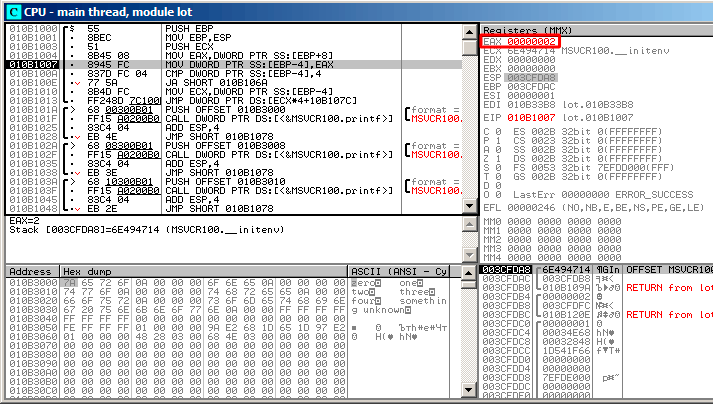
\includegraphics[scale=\FigScale]{patterns/08_switch/2_lot/olly1.png}
\caption{\olly: \RU{входное значение ф-ции загружено в}\EN{function's input value is loaded in} \EAX}
\label{fig:switch_lot_olly1}
\end{figure}

\clearpage
\RU{Входное значение проверяется, не больше ли оно чем}\EN{Input value is checked, if it's bigger than} $4$? 
\RU{Нет, переход по умолчанию (``default'') не будет исполнен}\EN{No, ``default'' jump is not 
taken}:
\begin{figure}[H]
\centering
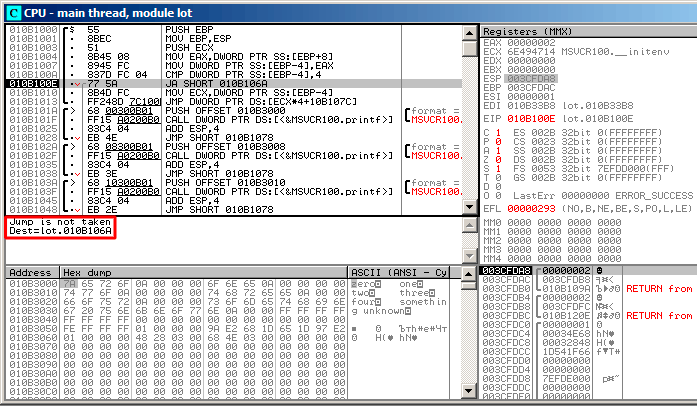
\includegraphics[scale=\FigScale]{patterns/08_switch/2_lot/olly2.png}
\caption{\olly: $2$ \RU{не больше чем}\EN{is no bigger than} $4$: \RU{переход не сработает}\EN{no jump is taken}}
\label{fig:switch_lot_olly2}
\end{figure}

\clearpage
\RU{Здесь мы видим}\EN{Here we see a} jumptable:

\begin{figure}[H]
\centering
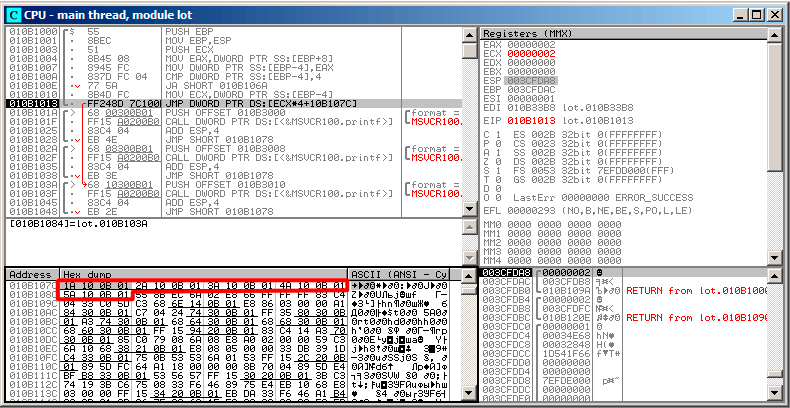
\includegraphics[scale=\FigScale]{patterns/08_switch/2_lot/olly3.png}
\caption{\olly: \RU{вычисляем адрес для перехода используя}\EN{calculating destination address using} jumptable}
\label{fig:switch_lot_olly3}
\end{figure}

\RU{Кстати, я кликнул}\EN{By the way, I clicked} ``Follow in Dump'' $\rightarrow$ ``Address constant'', 
\RU{так что теперь jumptable видна в окне данных}\EN{so now we see a jumptable in data window}. 
\RU{Это 5 32-битных значения}\EN{These are 5 32-bit values}\footnote{\EN{They are underlined by \olly because
these are also FIXUPs}\RU{Они подчеркнуты в \olly, потому что это также и FIXUP-ы}: \ref{subsec:relocs}, 
\RU{мы вернемся к ним позже}\EN{we will back to them later}}.
\ECX \RU{содержит сейчас}\EN{is} $2$\RU{, так что второй элемент (считая с нулевого) таблицы сейчас
будет использован}\EN{ now, so the second element (counting from zeroth) of table will be used}.
\RU{Кстати, можно также кликнуть}\EN{By the way, it's also possible to click} ``Follow in Dump'' $\rightarrow$ 
``Memory address'' \AndENRU \olly \RU{покажет элемент, который сейчас адресуется в инструкции \JMP}\EN{will
show the element \JMP instruction being address now}. 
\RU{Это}\EN{That's} \TT{0x010B103A}.

\clearpage
\RU{Переход сработал и мы теперь на}\EN{Jump occured and we now at} \TT{0x010B103A}: 
\RU{сейчас будет исполнен код выводящий строку}\EN{the code printing} ``two''\EN{ string will now be executed}:

\begin{figure}[H]
\centering
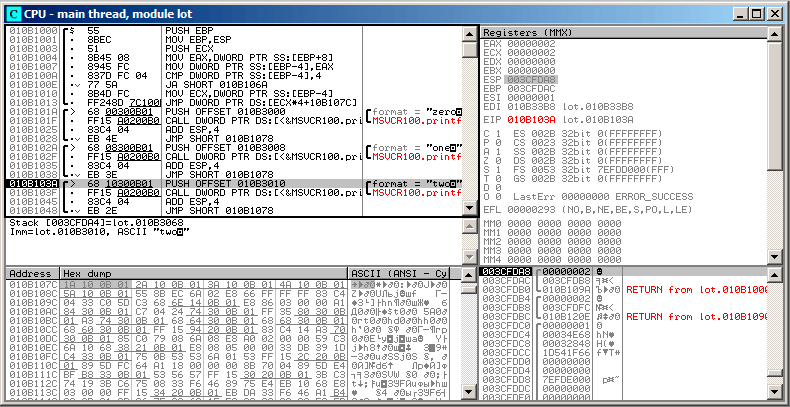
\includegraphics[scale=\FigScale]{patterns/08_switch/2_lot/olly4.png}
\caption{\olly: \RU{теперь мы на соответствующей метке}\EN{now we at corresponding} \IT{case:}\EN{ label}}
\label{fig:switch_lot_olly4}
\end{figure}
